%--------Preliminares
%--------Daniel Quinteros Céspedes
%--------23-09-2014

\chapter{Marco Te\'orico}
\label{cap:preliminares}

En el capítulo anterior se revisó el contexto general del problema, en el presente capítulo se dará paso a la explicación de los conceptos teóricos más relevantes que se relacionan con el trabajo expuesto en el presente documento. Algunos de ellos son la visión por computador, los elementos del procesos de detección de peatones y la sensibilidad espacial.

\section{Visión por computador}
\label{preliminares:cv}

Existen variadas definiciones sobre lo que se trata la visión por computador, \cite{mery2004} indica en su libro ``Visión por Computador'' algunas de las definiciones más relevantes enunciadas por expertos en el área.

\begin{itemize}
\item ``Ciencia que desarrolla las bases teóricas y algorítmicas para obtener información sobre el mundo real a partir de una o varias imágenes''~\citep{haralick1992}.
\item ``Disciplina que desarrolla sistemas capaces de interpretar el contenido de escenas naturales''~\citep{kennethr.1996}.
\item ``La Visión por Computador, que ha emergido como una disciplina propia basada principalmente en las matemáticas y ciencias de la computación consiste en hacer que un computador vea. Esto sin embargo es todavía un problema no resuelto\ldots''~\citep{hartley2003}.
\end{itemize}

La visión por computador o en inglés \textit{computer vision}, es entonces un campo de estudio dentro del área de la inteligencia computacional el cual se dedica al análisis y comprensión de la imágenes en general. El objetivo principal es emular la forma en la que el ojo humano (o el de otro ser vivo) es capaz de extraer e interpretar información de las imágenes, para esta tarea se vale del modelamiento matemático, la computación y la electrónica como principales herramientas. 

\begin{figure}[tp]
  \centering
  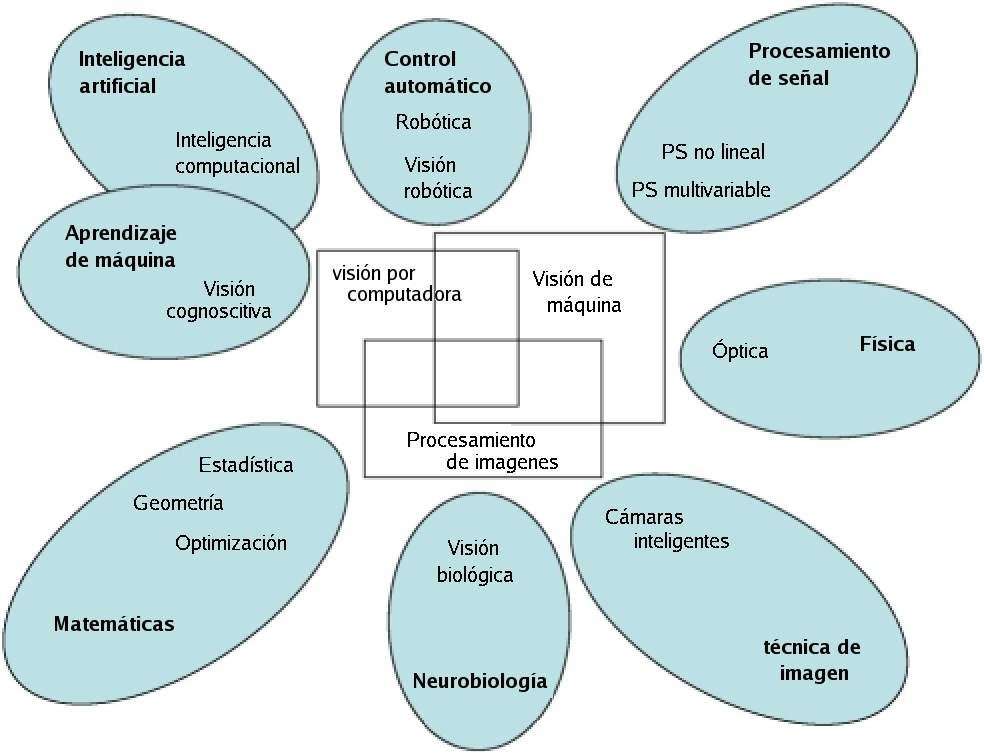
\includegraphics[scale=.3]{images/cv-context}
  \caption{\em Visión por computador y áreas afines.}  
  \label{fig:cvcontext}
\end{figure}

La visión por computador se encuentra rodeada de una gran cantidad de áreas de investigación de las cuales se ve nutrida (figura~\ref{fig:cvcontext}). Esta variedad de áreas afines implican una gran cantidad de potenciales aplicaciones relacionadas. Sin embargo, en general el proceso de procesamiento por el que pasan las imágenes es posible generalizarlo. Como se muestra en la figura~\ref{fig:cvprocess} el proceso se inicia con la adquisición de la imágenes obteniendo una imagen del objeto que se desea estudiar, luego en el pre-procesamiento se hace uso de algunos filtros digitales que permiten eliminar el ruido o eliminar el contraste con el objetivo de mejorar la calidad de esta, luego en la etapa de segmentación se realiza la identificación del objeto de estudio del resto de la imagen, en la medición o extracción de características se realiza una medición de los atributos de interés de la imagen y finalmente en la interpretación, se clasifica o etiqueta al objeto, es importante señalar el foco del presente documento se encuentra en esta última etapa y busca mejorar una parte del proceso de interpretación.

\begin{figure}[tp]
  \centering
  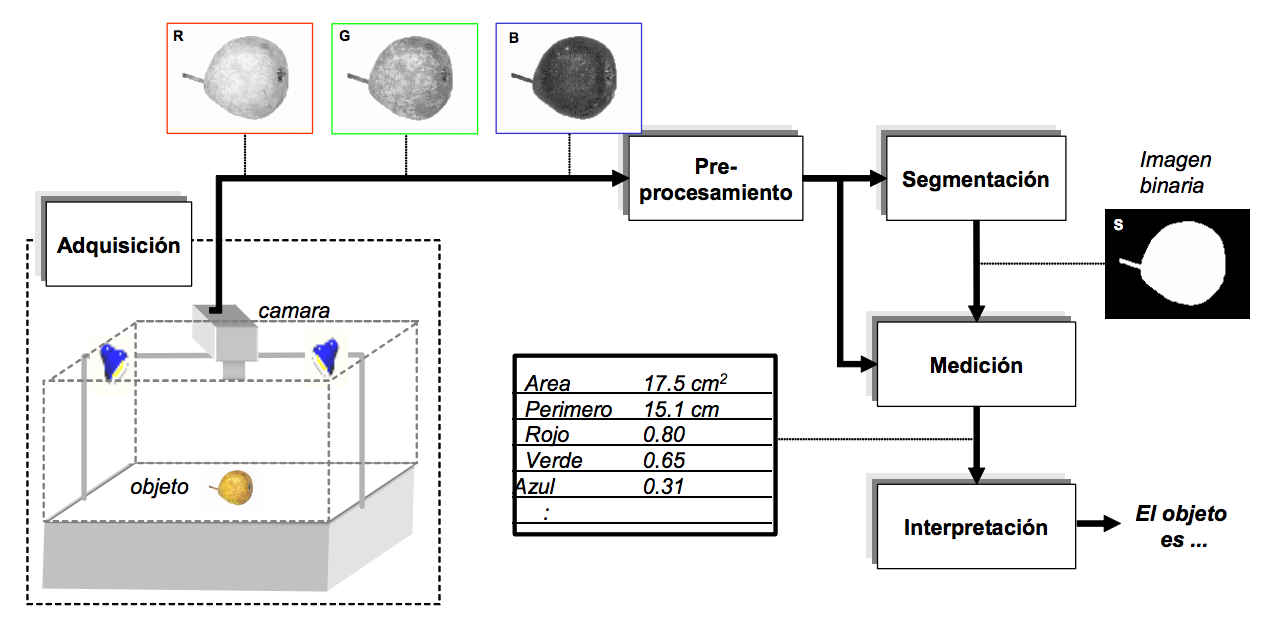
\includegraphics[scale=.3]{images/cv-system}
  \caption{\em Esquema de un proceso de análisis de imágenes.} 
  \label{fig:cvprocess}
\end{figure}

\section{Set de datos de peatones INRIA}
\label{preliminares:deteccion}

El set de datos de personas de INRIA, construido por \cite{dalal2005}, corresponde a una colección de imágenes de peatones en distintos formatos utilizado para el entrenamiento y pruebas del sistema solución. Está compuesto principalmente de imágenes provenientes de tres fuentes: el dataset de la Universidad Tecnológica de Graz, colecciones de imágenes personales del autor y Google Web Images. En todas estas imágenes aparecen personas de pie, y no todas las anotaciones son correctas, esto significa que para algunos casos, el recuadro de delimitación (\textit{bounding box}) puede estar desplazado respecto del objeto. En total el set de datos  contiene 
Las imágenes se presentan en dos formatos: las imágenes originales con sus archivos de anotaciones asociados, y las imágenes en positivo normalizadas a formato de 64x128 píxeles con las imágenes en negativo originales asociadas. Las imágenes originales están organizadas en una carpeta de entrenamiento y una carpeta de pruebas, y dentro de cada una de ellas, las carpetas pos, que contiene las imágenes en positivo, neg, que contiene las imágenes en negativo, y annotations, que contiene las anotaciones para las imágenes. Por su parte, las imágenes normalizadas se dividen en dos carpetas, pos y neg, las que siguen la misma lógica de nombres que las imágenes originales.
Utilizando este conjunto de datos, el sistema solución puede ser entrenado para así poder llevar a cabo la tarea de detección de personas. En el siguiente paso se revisará información sobre los algoritmos utilizados para extraer información de las imágenes

\section{Características de las imágenes}
\label{preliminares:caract}

Para cualquier tarea de detección es necesario obtener información de la imagen que permita diferenciar un objeto de otro o una persona de otra, en este punto entran las técnicas de extracción de características que entregan como resultado simbología que permite a un computador interpretar lo que esta ``viendo''. En un escenario ideal estas características deberían representar a un objeto en la imagen y permanecer constante durante cambios de iluminación, cambios de punto de vista o cambios en el borde de los objetos. Para lograr esto se han desarrollado distintos enfoques, \cite{dalal2006} indica que estos enfoques se pueden agrupar en dos categorías o enfoques diferentes. La primera categoría, representaciones dispersas incluye detección basada en puntos, en fragmentos de la imagen y en partes. La segunda categoría es la de representaciones densas y utiliza la intensidad de la imágenes o gradientes.

\subsection{Representaciones locales dispersas}
\label{caract:dispersas}

Las representaciones dispersas intentan describir las características de la imagen utilizando regiones localizadas de la imagen. Comúnmente estas regiones son seleccionadas utilizando uno de dos enfoques: detección de puntos clave o detección de partes. A continuación se revisará brevemente ambos enfoques.

\subsubsection{Detectores de puntos clave (\textit{keypoints})}

La idea esencial detrás de los detectores basados en puntos clave (\textit{keypoints}) es que son capaces de seleccionar regiones estables y fiables de la imagen las cuales contienen información muy representativa del contenido local de la imagen. Entonces, los detectores cuyo enfoque esta basados en puntos clave tienen por objetivo extraer de la imagen un pequeño conjunto de puntos sobresalientes de la imágenes o puntos de interés, estos puntos de interés son procesados para obtener vectores de características de ellos los que a su vez permiten, finalmente, la construcción del detector. Las principales ventajas del uso de detectores basado en puntos clave es su tamaño, el cual es considerablemente más pequeño que la cantidad de píxeles en la imagen lo que permitiría un procesamiento más rápido en las últimas etapas del proceso de detección. En general el desempeño de los detectores basados en puntos clave depende de que tan informativos sean los puntos encontrados y si para una clase determinada es posible encontrar estos puntos de una forma fiable, precisa y repetible. Algunos de los enfoques más populares \citep{gupta2008} en cuanto a los puntos clave son \textit{Scale Invariant Feature Transformation} (SIFT) \citep{Lowe2004}, el cual resuelve unos de los problemas más relevantes de la detección por puntos clave: la invariabilidad frente al escalado; \textit{Gradient Location and Orientation Histogram}~(GLOH)~\citep{Mikolajczyk2005}, este descriptor es una mejora de SIFT que busca mejorar la robustez y el grado de diferenciación; \textit{Shape context}~\citep{Belongie2002}, es una manera de describir la forma que permite medir la similitud y recuperar la correspondencia de los puntos; \textit{Speeded Up Robust Features} (SURF) \citep{Bay2006}, es esencialmente un algoritmo inspirado en SIFT y pensado para mejorar el tiempo de computo; PCA-SIFT~\citep{Ke2004}, es también una mejora de SIFT que esta vez utiliza análisis de componentes principales (PCA) haciendo más compacto al descriptor.

% ***SAV: no entiendo el párrafo siguiente !!!
Aún cuando la utilización de detectores basados en puntos clave se encuentra ampliamente extendida dentro del problema de detección de objetos, presenta un problema característico. Este tipo de detectores se encuentran diseñados para encontrar repetidamente un mismo objeto en una imagen por lo surgen problemas cuando el objeto se generaliza en clases o categorías.


\subsubsection{Detectores basados en partes o extremidades}

La detección basada en partes así como la basada en puntos clave también tiene un uso extendido en los sistemas de detección de peatones. Para este caso en particular de detección existen también distintos enfoque. Sin embargo, la ideea principal detrás de la detección basada en partes es que las partes o extremidades pueden ser representadas de forma geométrica. Existen enfoques en los cuales se asume que cada parte de cuerpo como, antebrazo, brazo, torso, etc.  puede representarse bien utilizando un cilindros \citep{Ramanan2003}. Otros tipos de construcciones geométricas también han sido utilizadas para este fin, por ejemplo usando detección de bordes para obtener modelos relativos de la extremidades. Otros enfoques utilizando este tipos de descriptores son los detectores de extremidades 3D \citep{Sigal2003}. En general estos descriptores funcionan bien, sin embargo presentan algunos problemas, pues la simplicidad de la representaciones geométricas con lineas son difíciles de extrapolar a la complejidad del mundo real.


\subsection{Representaciones densas de las regiones de una imagen}
\label{caract:densas}

Las representaciones locales tienen en general una ventaja respecto de la velocidad de cómputo. Sin embargo, al ser locales pueden perder la perspectiva, por lo que es importante revisar su contrapartida, en este caso, las representaciones densas. En general estas representaciones obtienen una cantidad de características muy grande incluso tantas como píxeles haya para una imagen entera o un ventana de detección obteniendo vectores descriptores con una alta dimensionalidad el cual puede ser utilizado para realizar un clasificación. 
A continuación se explicarán algunos enfoques relacionados con este tipo de representaciones, que están generalmente basadas en la utilización de intensidades de la imagen, gradientes u operadores diferenciales.

\subsubsection{Regiones basadas en la intensidad de la imagen}

Aún cuando en general los detectores basados en la intensidad de la imagen han sido utilizados principalmente para la obtención de puntos clave en representaciones locales dispersas, también existen algunos ejemplos en representaciones densas. Según \cite{dalal2006}, una de los primeras propuestas de este tipo de descriptores corresponden a las realizadas por \cite{Sirovich1987} y \cite{Turk1991} utilizando intensidades simples de la imagen. Este enfoque se conoce como \textit{``eigenfaces''} y el mismo autor señala también la existencia de otros dos enfoques. El primero para el desarrollo de un sistema de reconocimiento de rostros cuyo proceso realiza un ajuste  la luminosidad de la imágenes con una ecualización del histograma para luego clasificar utilizando una red neuronal \citep{Rowley1998}. El segundo caso utiliza un algoritmo de tipo goloso que basado en su patrón de intensidad selecciona los fragmentos (generados aleatoriamente) más importantes de un objeto en la imagen \citep{Ullman2001}.

\subsubsection{Detectores basados en gradiente}

Dentro de los detectores basados en gradiente es posible encontrar uno de los más ampliamente utilizados métodos para la detección de peatones propuesto por \cite{dalal2005}. Este descriptor se conoce como \textit{Histogram of Oriented Gradients} (HOG). Este algoritmo toma secciones en bloque superpuestas de una misma imagen y calcula la orientación y magnitud del gradiente para cada una conjugando todo en un histograma de gradientes orientados. Posterior a su aparición se han propuesto mejoras como la de \cite{Zhu2006}, que permiten mejorar su velocidad de cómputo, o la de \cite{Felzenszwalb2009}, que introduce un modelo basado en partes con una estructura estrella definido por un filtro ``raiz'' además de filtros para las partes con un modelo de deformación asociado. Otros enfoques dentro de los descriptores basados en gradiente que son importantes de mencionar son los de \cite{Mikolajczyk2004a} y \cite{Ronfard2002}. El primero diseñó un descriptor especialmente para la detección de personas utilizando para ello un modelo del cuerpo en siete partes, cabeza de frente y perfil, torso, brazos y piernas. El segundo desarrolló un descriptor para un cuerpo articulado basado en partes utilizando un clasificador SVM de extremidades construido sobre filtros gaussianos de primer y segundo orden.

\subsubsection{Detectores basados en \textit{wavelets}}

El último grupo de clasificadores son los clasificadores basados en (\textit{wavelets}). Algunos ejemplos conocidos de este tipo de descriptores son \cite{Papageorgiou2000}, \cite{mohan2001} y \cite{viola2001}. Estos descriptores de representación densa en general utilizan operadores parecidos al wavelet de Haar,  propuesto por primera vez por Alfred Haar, ``convirtiéndose en el primer referente a las wavelets, al trabajar con funciones de soporte compacto, es decir, que se anulan fuera de un intervalo finito. Desafortunadamente la wavelet de Haar no es continuamente diferenciable, por lo que sus aplicaciones se vieron limitadas'' \citep{FernandezSarria2007a}. Es también destacable el hecho de que el trabajo \cite{Papageorgiou2000} fue uno de los primeros en proponer un enfoque de ventana deslizante para la detección utilizando una máquina de vectores de soporte sobre un diccionario a múltiples escalas de wavelets de Haar.

\section{Clasificadores}
\label{preliminares:clasif}

En la sección \ref{caract:dispersas} se analizaron algunos de los principales métodos de extracción de características utilizados en la detección de personas. Ahora es necesario revisar las propuestas en materia de algoritmos de clasificación. Los clasificadores son algoritmos que permiten asignar un objeto sin clasificar a una clase o categoría determinada. Los algoritmos de clasificación en general es posible agruparlos en dos categorías diferentes \citep{ng2002} modelos generativos y discriminativos. Los modelos generativos aprenden un modelo de probabilidad conjunta, \textit{p(x,y)} donde \textit{x} son las entradas e \textit{y} las etiquetas de la clase, las predicciones se realizan utilizando el teorema de Bayes para calcular la probabilidad condicional o posterior \textit{p(y\textbar x)} seleccionando la etiqueta \textit{y} con la mayor probabilidad. Los modelos discriminativos de clasificación aprenden directamente un modelo de la probabilidad condicional \textit{p(y\textbar x)} o aprenden de un mapa directo desde las entradas \textit{x} a las etiquetas \textit{y}.

\subsection{Modelo generativo}

En los problemas de detección el modelo generativo es, en general, menos utilizado que el modelo discriminativo. Sin embargo, es posible encontrar algunos ejemplos como el trabajo de \cite{Vidal-Naquet2003} en el cual se utiliza un clasificador Naïve Bayes y además se muestra que usar un árbol de clasificación basado en redes Bayesianas no tiene una gran mejora respecto del proceso de clasificación. En el mismo trabajo se plantea también un tipo de descriptor utilizando fragmentos de imagen y se compara con descriptores de tipo wavelet mostrando un mejora apreciable. Otro ejemplos de esto son \cite{Weber2000} y \cite{Fergus2003} quienes también utilizan modelos Bayesianos, pero incluyen un sistema que usa una razón de probabilidades \textit{p(y\textbar 1)~/~p(1\textbar 0)} para realizar la clasificación.

\subsection{Modelo discriminativo}

Para los problemas de detección de peatones los clasificadores con modelos dsicriminativos son más utilizados que los con modelo generativo. Sin embargo su variedad no es muy amplia ya que existen dos tipos de clasificadores que se han transformado en el \textit{"gold standard"} para los problemas de este tipo \cite{dollar2012}. Estos son las máquinas de vectores de soporte (SVM) y algoritmos de boosting. A continuación se revisarán ambos tipos de clasificación.

\subsubsection{Máquinas de vectores de soporte (SVM)}

La idea esencial detrás de SVM es que dado un conjunto de datos el algoritmo encuentre un hiperplano tal que separe los datos de cada clase (peatón y no peatón) en forma óptima. En caso de no encontrarse el óptimo en una determinada dimensión, el SVM permite proyectar estos puntos a una dimensión superior. Actualmente las SVM son ampliamente utilizadas para resolver problemas de clasificación, especialmente las SVM de tipo lineal aunque existen buenos ejemplos de otros tipos de SVM como el de \cite{Maji2008} quien plantea una mejora de desempeño con un método basado en \textit{histogram intersection kernel SVM}.
Las SVM lineales no solo proveen buenos resultados en términos de la detección respecto de otros clasificadores, si no que también su velocidad permite que puedan ser utilizados para la realización de aplicaciones en tiempo real. Uno de los trabajos más importantes sobre detección de peatones es el de \cite{dalal2005} y \cite{dalal2006} en el cual desarrollan el descriptor HOG y utilizan un SVM lineal para realizar el proceso de clasificación. Por otro lado uno de los primeros en incluir un clasificador SVM con el enfoque de la ventana deslizante fueron \cite{Papageorgiou2000}. 

% ***SAV tal vez seria bueno mucho antes explicar lo de la ventana deslizante en el espacio xy y en escalas de tal manera que el método que se usa para detección quede claro (o sea el de una búsqueda exhaustiva por la imagen a distintas escalas - como causa de entrenar un clasificador a una escala normalizada. Luego, el problema de sensibilidad queda más claro). Por eso yo lo colocaría en el primer capítulo de introducción o lo antes posible en este capítulo ***DQ Revisado

Las máquinas de vectores de soporte son quizá el más popular clasificador utilizado para la detección de peatones y objetos en general, sin embargo tienen una competencia muy estrecha con los algoritmos de boosting y en especial Adaboost el cual se expone a continuación.

\subsubsection{AdaBoost}

Los algoritmos de Boosting fueron desarrollados para combatir la ``maldición de las dimensiones''~\citep{bellman1961adaptive}, este concepto hace referencia a un conjunto de problemas que surgen cuando se analizan problemas en espacios de características con un alta dimensionalidad. 
Este tipo de algoritmos introducidos por primera vez por \cite{Schapire1990}, indicando que era posible construir un aprendiz fuerte a partir de muchos aprendices débiles. Un aprendiz débil es un clasificador que es levemente mejor en su clasificación que "lanzar una moneda al aire", es decir que su tasa de error es levemente inferior a 0.5 en una clasificación binaria, mientras que un aprendiz fuerte es un clasificador que obtiene resultados positivos con una alta probabilidad \citep{Kearns1994}. Utilizando estos principios \cite{Freund1995} desarrollaron un algoritmo conocido como AdaBoost (Adaptative Boosting). Este algoritmo es hoy ampliamente utilizado en problemas de detección como por ejemplo \cite{viola2001}, \cite{dollar2009a}, \cite{Dollar2010} y \cite{wojek2008}. 

\section{\textit{Non-Maximal Supression}}
\label{preliminares:nms}

% ***SAV falta ...***DQ Revisado

\textit{Non-Maximal Supression} (NMS) es un método ampliamente utilizado en los algoritmos de detección de objetos para realizar el post procesamiento de las clasificaciones realizadas. El objetivo del método consiste en encontrar todos los máximos locales en la clasificación. Inicialmente el término se utilizó en el contexto de la detección de bordes para reducir el grosor de éstos a líneas más finas. Este tipo de \textit{Non-Maximal Supression} funciona en una dimensión perpendicular al borde. 
En general el algoritmo tomará un conjunto de elementos en una vecindad y comprobará cuál de éstos es mejor que sus vecinos. Realizando esto, es posible encontrar detecciones únicas en una imagen. Para la etapa de post procesamiento NMS se utilizas como un método para realizar la ``fusión'' de las múltiples detecciones. Para esto el algoritmo debe tener en cuenta los siguientes principios.

\begin{itemize}
\item Mientras mayor sea la respuesta del clasificador para una detección, mayor probabilidad de encontrar un verdadero positivo en la vecindad.
\item Mientras más superpuestas se encuentren las detecciones en una vecindad, mayor probabilidad de encontrar un verdadero positivo.
\item Las detecciones sobrepuestas en una pequeña vecindad deben ser fusionadas, a menos que la detección ocurra a escalas muy distintas.
\end{itemize}

En la imagen \ref{fig:nms} es posible observar un ejemplo del resultado obtenido de aplicar NMS como método de post procesamiento.

\begin{figure}[H]
  \centering
  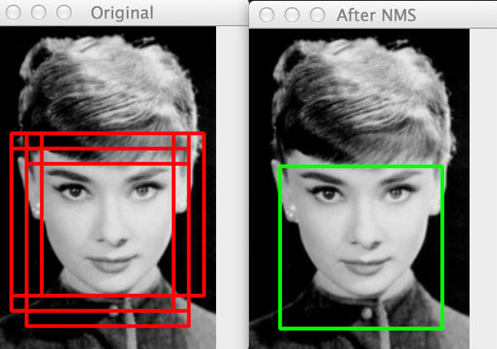
\includegraphics[scale=.3]{images/nms}
  \caption{\em Antes y después de NMS. Adaptado de \cite{Rosebrock2014}} 
  \label{fig:nms}
\end{figure}


\section{\textit{Extreme Programming} (XP)}
\label{preliminares:xp}

Es importante presentar antecedente para caracterizar la metodología que hace de base para la adaptación realizada en el presente trabajo. Extreme Programming consiste, en palabras de su autor, \cite{Beck1999}, a través de su libro \textit{``Extreme Programming Explained: Embrace Change''} en ``una disciplina del negocio de desarrollo de software que enfoca a todo el equipo en metas comunes y alcanzables''. También lo define como ``un estilo de desarrollo de software que se enfoca en una excelente aplicación de técnicas de programación, comunicación clara y trabajo en equipo''. Es, el en fondo, una metodología ágil de desarrollo de software, enfocada principalmente en generar valor agregado a la solución.
El enfoque de XP se centra en ``hacer lo que necesitas hacer para crear valor para el cliente'' \citep{Beck1999}. De esta afirmación se puede desprender que esta metodología se enfoca directamente en el proceso del desarrollo del software, donde ``la programación es la actividad clave''. El espíritu de la metodología es equivalente a conducir un auto (en palabras del autor): no se trata de llevar el auto en la dirección correcta, sino que de poner atención de manera constante y corregir la dirección del auto apenas sea necesario. El desarrollo es guiado a través de cinco valores: comunicación, simplicidad, retroalimentación, valentía y respeto. Para llevar los valores a la práctica, XP se sirve de los principios, que guían las decisiones relativas al proyecto.
\begin{itemize}
\item La retroalimentación: el desarrollo está guiado por pruebas. Cuando se reporta un error en el sistema, debe adjuntarse el caso de prueba fallido. Se postula que el tiempo entre una acción y su retroalimentación debe ser mínimo a fin de poder aprender y realizar cambios si es necesario. Se conversa de manera constante con el cliente, a fin de asegurarse que el producto en desarrollo concuerda con la idea en mente que tiene el cliente de éste y sus expectativas, toda vez que se asume que el cliente no tiene – desde un principio – un concepto absolutamente claro y entendible de lo que necesita, esto es, el equipo de desarrollo no podrá diseñar exactamente lo que el cliente imagina sin su constante retroalimentación sobre el producto que se está elaborando.
\item La simplicidad: para todo problema su solución es extremadamente simple. El código debe diseñarse de tal forma que sea lo más simple posible.
\item La aceptación del cambio: no debe verse al cambio como un elemento a evitar, tendiendo a programar todo con el fin de hacerlo reusable. Si el cliente necesita cambios en el producto en desarrollo, el equipo debe estar dispuesto a asumirlos de manera activa con el fin de poder implementarlos lo más pronto posible.
\end{itemize}
 
Al ser una metodología ágil, XP se orienta más hacia el cambio constante que a una planificación previa extensa y posteriormente inflexible. Beck afirma en su libro que XP puede funcionar con equipos de cualquier tamaño, no obstante cuando fue diseñado su enfoque estaba orientado hacia equipos de tamaño pequeño de no más de diez personas, evolucionando desde su aplicación en desarrollos internos y de menor categoría a ser la metodología principal de desarrollo del software.
XP se centra en llevar al extremo aquello que es considerado bueno, de ahí la razón de ser de la palabra ``extrema'' para el nombre de la metodología. Alienta al lanzamiento frecuente de \textit{releases}, en términos de horas, no en semanas o meses. Establece que el proceso de desarrollo debe hacerse en pares, donde una persona programa y la otra le asiste, revisando aquello que está siendo programado y contribuyendo con ideas. Estos puestos son periódicamente intercambiables. Todos los involucrados deben probar el producto de manera constante: si se detecta una falla, el reporte del problema involucra adjuntar el caso de prueba fallido. Estos \textit{releases} deben ser pequeños incrementos, cuidando además de integrar continuamente. Para que el desarrollo del software cumpla con el valor de la comunicación, el equipo de desarrollo debe definir estándares de programación que sean entendibles por todos: el individualismo y la idiosincrasia de distintos estilos de programación no contribuye al beneficio del grupo, es sólo la manifestación de un estilo individual, que dificulta la comunicación entre los integrantes del equipo al no existir una estructura y estilos comunes de desarrollo del código que puedan ser entendibles rápidamente por todo el equipo. Debe pensarse que todo el equipo es propietario del código que está en desarrollo, por lo tanto, las parejas que están programando una funcionalidad pueden, en teoría, pasar a trabajar rápidamente en otra funcionalidad sin tener que demorarse demasiado en interpretar cuál fue la forma en que se implementó tal funcionalidad por parte de la pareja anterior, por lo tanto, el desarrollo de las funcionalidades se vuelve independiente del programador, sobre todo, del que la haya implementado en primer lugar.
Beck señala que los elementos que diferencian a XP de otras metodologías son.
\begin{itemize}
\item Sus ciclos de desarrollo cortos, que dan como resultado una retroalimentación temprana, concreta y continua.
\item Su aproximación desde la planificación incremental, que rápidamente deriva en un plan general que se espera que evolucione a lo largo de la vida del proyecto.
\item Su habilidad para programar de manera flexible la implementación de funcionalidades, respondiendo a las necesidades cambiantes del negocio.
\item Su dependencia en:
\subitem - Pruebas automatizadas escritas por programadores, clientes y probadores para monitorear el progreso del desarrollo, permitir la evolución del sistema y detectar defectos de manera temprana.
\subitem - La comunicación oral, pruebas y el código fuente para comunicar la estructura e intención del sistema.
\subitem Un proceso de diseño evolutivo que dura tanto como dure el sistema.
\subitem - La colaboración cercana de personas comprometidas con talento común y corriente.
\subitem - Prácticas que funcionan tanto con los instintos a corto plazo de los miembros del equipo y los intereses a largo plazo del proyecto. 
\end{itemize}


\section{Conclusiones del capítulo}
\label{preliminares:conclusiones}

% ***SAV falta ***DQ Revisado

El marco teórico expuesto pretende contextualizar al lector sobre los tópicos más importantes tratados en el presente trabajo de título. Se trata tanto conceptos generales (Visión por computador, Características, Clasificadores) como específicos (SVM, NMS, Adaboost). El conocimiento de estos conceptos y mejor su aplicación por parte del lector facilitará la comprensión del los puntos desarrollados en los capítulos sucesivos. Si fuera necesario obtener mayor información de los conceptos aquí expuestos revisar las referencias citadas, cuyo detalle se encuentra al final del cuerpo principal del presente documento. 

Un resumen breve de los puntos tratados en este capítulo es el que sigue. En primer lugar, se ha revisado el concepto de visión por computador, que es el área general en la que este trabajo se enfoca y que consiste en palabras simples de emular el sentido de la percepción visual de los seres vivos a través de un computador, permitiendo gracias a esto, detectar elementos de interés dentro de imágenes. También se caracterizó el conjunto de datos utilizado por los clasificadores a fin de medir la calidad de sus detecciones; siendo este conjunto único para todos estos clasificadores. Posteriormente se ha detallado cómo las características de los objetos son extraídas de la imágenes a través de algoritmos denominados, descriptores. Se menciona además a los clasificadores los cuales evaluarán la información obtenida en por los descriptores con el objetivo de asignar una clase o categoría, en este caso peatón o no peatón. Posteriormente se trata el método de \textit{Non-maximal supression} que permitió realizar el procesamiento de las imágenes ya clasificadas. Y por último, se ha hecho referencia a \textit{Extreme Programming}, que corresponde a la metodología de desarrollo de software con la que se implementará la solución al problema propuesto.




